\documentclass[openany]{book}

\usepackage{titlesec}

\titleformat{\chapter}[display]
{\normalfont\huge\bfseries}{}{0pt}{\Huge}

% \newtheorem{lemma}{Lemma}[section]

\usepackage{fancyhdr}
\usepackage{lipsum}
\pagestyle{fancy}
\fancyhf{}
\fancyhead[LE,RO]{\leftmark}

\usepackage{amsthm}
\usepackage{amssymb}
\usepackage{amsmath}
\usepackage{graphicx}
\usepackage{subcaption}
\usepackage{amsfonts}
\usepackage{mathtools}
\usepackage[backend=bibtex]{biblatex}
\usepackage{graphicx}
\usepackage{float}
\usepackage[a4paper, margin=1in]{geometry}
\usepackage{amssymb}

\title{Statistical Analysis}
\date{\today}
\author{
	V.S.S. Vardhan : 23b0909 \\
	Shasank Reddy P : 23b1015 \\
	Sree Vamshi Madhav Nenavath: 23b1039 \\
}

\begin{document}
	
	\maketitle
	\tableofcontents

    \theoremstyle{plain}
	\newtheorem{theorem}{Theorem}
    \newtheorem{lemma}{Lemma}
	

	
	% -----------------------------------------------------------------------------------------------
	
	% \chapter{Question 3}

    % \section*{Instruction for python code}

    % \begin{itemize}
    %     \item use ``\textbf{python3 3.py}'' to run all the tasks at once or
    %     \item use ``\textbf{python3 3.py 3@}'' @=[a,b,c,d,e,f] to run subparts
    %     \item use ``\textbf{python3 3.py bonus}'' to run bonus task
    % \end{itemize}

    % \section{Task A}
    %     The $ith$ moment of a random variable is defined as $\mu_i = E[X^i]$ which can be calculated by the numpy function 
    %     mean $ \mu_i = np.mean(data**i)$. 
    
	% \section{Task B}
	% We can plot a histogram using \textbf{\textit{matplotlib.pyplot}} plt.hist(data,bins=100,label)  
	% \begin{figure}[H]
	% 	\centering
	% 	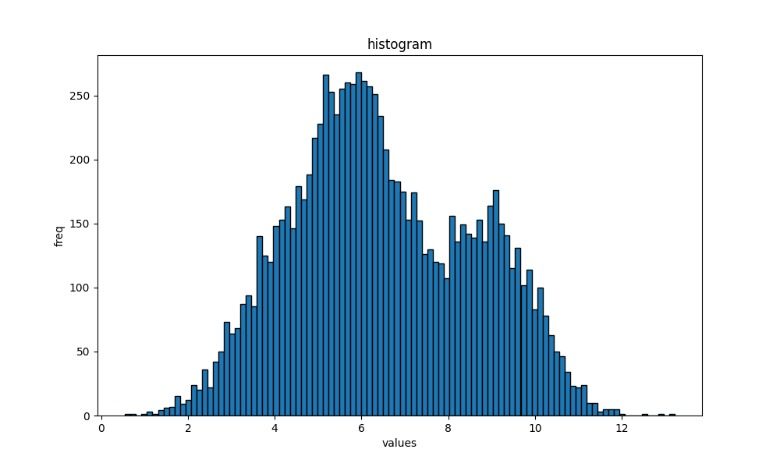
\includegraphics[width=1.0\textwidth]{photos/histogram.jpeg}
	% 	\caption{Histogram of the given dataset.}
	% 	\label{fig:sample}
	% \end{figure}
	
	% We can clearly observe that the mean should be around 6  from the histogram. 
	
	% \section{Task C}
	% The first two moments of a binomial distribution $B(n,p)$ are given by
	
	% \[ \mu_1^{bin} = E[X] = np \]
	% \[ \mu_2^{bin} = E[X^2] = var(X) + (E[X])^2\]
	% \[ \mu_2^{bin} = np(1-p) + (np)^2\]
	
	% We obtain the values of n*,p* by equating $\mu_1^{bin}$ and $\mu_2^{bin}$
	% to original moments of the dataset. We should round to the nearest int whichever reduces the error .\\
	
	% We can use the $fslove$ to do this; fsolve takes k equations and k parameters(with initial guess value) as arguments. 
	% and gives the values of parameters which best satisfy the equations as output.
	
	% \textit{formulae\_bin\(var\)} function gives the equatins to \textbf{solutions()}  which uses fsolve to find n,p, upon running the program we get \\
	% \[ n^* = 20\]
	% \[ p = 0.32968652963743666\]
	
	% Then, plot the binomial distribution over the histogram. By usnig  $ numpy.linspace$ and $scipy.stats.binom.pmf$ to generate the PMF of the distribution.
	
	% \section{Task D}
	% For Gamma distribution with parameter $k$ and $\theta$ $f(x;k,\theta)$ which is given by:
	% \[ f(x;k,\theta) = \frac{1}{\theta^{k}\Gamma{(k)}}.x^{k-1}.e^{-\frac{x}{\theta}} \]
	% where $\Gamma(k) = \int_0^\infty t^{k-1} e^{-t}dt$\\
	% The nth moment  of gamma function is given by
	% \[E[X^n] = \theta^{n}.\frac{\Gamma{(k+n)}}{\Gamma{(k)}}\]
	% \[ E[X^n] = \theta^{n}.\prod_{i=1}^{n}(k+i-1)\]
	
	% The first two moments $\mu_1^{gamma}$ and $\mu_1^{gamma}$ are $k \cdot \theta$ and $\theta^2 \cdot k \cdot (k+1)$ respectively. 
	% On solving these equations using $fsolve$ in the same manner as above but here we need not round off n to n integer because both $k,\theta$ are real; the estimated values of $k^*$, $\theta^*$ are
	
	% \[ k^* = 9.691205541211048 \] 
	% \[ = 9.69\]
	% \[ \theta^{*} = 0.6703134703624437  \]
	% \[ = 0.67\]
	
	% The plot we get using this gamma function is in \textbf{\textit{3d.png}}       
	% \section{Task E}
	% The likelihood function is a tool for comparing distribtuions over a datset, We can conclude which distribution suits the dataset better by comparing the likelihood/ log-likelihood values
	% the larger the likelihood/log-likelihood values it is a better fit.\\
	% We start by defining two functions log\_likilehood\_bin and log\_likelihood\_gamma , we first calculate normal likelihoods by using $binom.pmf(rounded\_data,n,p)$ and $gamma.pdf(data,k,scale=\theta)$
	% and then use np.log and np.mean to find the log-likelihoods and finally compafre these values and deduce the better fit.
	% \\
	% The log likelihood values turnout to be 
	% \[ log\_likelihood\_bin = -2.157068\] 
	% \[ log\_likelihood\_gamma =-2.1608217\]
	% Which indicate that Binomial distribution is a better fit 
	% \section{Task F}
	% Here, we will repeat what we have done in task D but for a Gaussin Mixture model, we are given that our GMM consists of 2 gaussian distributions with variances 1 each.
	% By solving equations genertaed by equating the first four moments we can find the values of parameters $\mu1,\mu2,p1,p2$ .
	
	% Next we calculate the log likelihood of the gaussian mixture mix by first calculating the PDF using $scipy.stats.norm.pdf$ and $np.mean(np.log)$ and we calculate the negative of the it.
	% negative log likelihoood is often calculated and is minimized to find the best fit curve.
	
	% After running all the programs we get the parameters
	% \[ \mu_1^* , \mu_2^*  =  (5.12960769428759,8.774363054417705)\]
	% \[ p1,p2 = (0.6118740341616438,0.382645651192205)\]
	
	% and the nll of gmm is $2.183038744$
	
	% By this we can conclude that binomial is a better fit than the gamma and gmm distribution.
	% And gamma is better fit than the GMM distribution. 
	
	
	% \section{Bonus Task}
	
	% Using the same approach as above i.e; equating the moments and solving them to find the unknown parameters is not efficient and we will not obtain close values. Instead we employ an algorithm called \textbf{ expectation maximization}  to find the parameters of the GMM. A general expectation maximisation algorithm involves 2 major steps :the Expectation Step (E) and the Maximisation step (M) . These steps repeat until convergence.
	
	% \subsection*{Step-by-Step Procedure}
	
	% \subsubsection*{Step 1: Initialize Parameters}
	
	% First, the parameters for each of the \( K \) components of the mixture model must be initialized. These parameters include:
	
	% \begin{itemize}
	% 	\item \( \mu_k \) (the \textbf{mean} for each component),
	% 	\item \( \sigma_k \) (the \textbf{variance} for each component),
	% 	\item \( \pi_k \) (the mixing coefficient(\textbf{wieghts}) for each component, where \( \sum_{k=1}^{K} \pi_k = 1 \)).
	% \end{itemize}
	
	% These can be initialized using random values, k-means clustering, or any other heuristic.
	
	% \subsubsection*{Step 2: Expectation Step (E-step)}
	
	% In the E-step, we calculate the responsibility \( \gamma_{ik} \), which represents the probability that a given data point \( x_i \) was generated by component \( k \). This step involves computing the posterior probabilities using the current parameters:
	
	% \[
	% \gamma_{ik} = \frac{\pi_k \mathcal{N}(x_i \mid \mu_k, \sigma_k^2)}{\sum_{j=1}^{K} \pi_j \mathcal{N}(x_i \mid \mu_j, \sigma^2_j)}
	% \]
	
	% Where:
	% \begin{itemize}
	% 	\item \( \gamma_{ik} \) is the responsibility of component \( k \) for data point \( x_i \),
	% 	\item \( \pi_k \) is the mixing coefficient for component \( k \),
	% 	\item \( \mathcal{N}(x_i \mid \mu_k, \Sigma_k) \) is the Gaussian probability density function for component \( k \) with mean \( \mu_k \) and covariance matrix \( \Sigma_k \).
	% \end{itemize}
	
	% This step computes the expected value of the latent variables (i.e., which Gaussian generated each data point).
	
	% \subsubsection*{Step 3: Maximization Step (M-step)}
	
	% In the M-step, we update the parameters \( \mu_k \), \( \sigma_k \), and \( \pi_k \) based on the responsibilities \( \gamma_{ik} \) computed in the E-step. The update equations are as follows:
	
	% \begin{itemize}
	% 	\item Update the means \( \mu_k \):
	% 	\[
	% 	\mu_k = \frac{\sum_{i=1}^{N} \gamma_{ik} x_i}{\sum_{i=1}^{N} \gamma_{ik}}
	% 	\]
	% 	where \( \mu_k \) is the weighted average of the data points assigned to component \( k \).
		
	% 	\item Update the variances \( \sigma_k \):
	% 	\[ \sigma^2_k = \frac{\Sigma_{i=1}^{N} \gamma_{ik}(x_i - \mu_k)^2}{\Sigma_{i=1}^{N} \gamma_{ik}}
	% 	\]
	% 	where \( \Sigma_k \) is the weighted covariance of data points assigned to component \( k \).
		
	% 	\item Update the weights \( \pi_k \):
	% 	\[
	% 	\pi_k = \frac{1}{N} \sum_{i=1}^{N} \gamma_{ik}
	% 	\]
	% 	where \( \pi_k \) is the fraction of data points assigned to component \( k \), ensuring that \( \sum_{k=1}^{K} \pi_k = 1 \).
	% \end{itemize}
	
	% These updates maximize the expected complete log-likelihood given the current responsibilities.
	
	% \subsubsection*{Step 4: Check for Convergence}
	
	% After each E-step and M-step, we check if the algorithm has converged. The convergence criterion can be based on one of the following:
	
	% \begin{itemize}
	% 	\item The change in log-likelihood is below a small threshold,
	% 	\item The parameters (means, variances, and weights) stop changing significantly between iterations,
	% 	\item A pre-set maximum number of iterations has been reached.
	% \end{itemize}
	
	% If the algorithm has not converged, return to the E-step and repeat the process.
	
	% \subsection*{Mathematical Objective}
	
	% The EM algorithm seeks to maximize the log-likelihood function:
	% \[
	% \log L(\theta) = \sum_{i=1}^{N} \log \left( \sum_{k=1}^{K} \pi_k \mathcal{N}(x_i \mid \mu_k, \sigma^2_k) \right)
	% \]
	% where \( \theta = \{\mu_k, \sigma_k, \pi_k \} \) represents the parameters of the model.
	
	% Since directly maximizing this log-likelihood is difficult due to the latent variables (which Gaussian generated each data point), the EM algorithm iteratively maximizes a lower bound on this log-likelihood.
	
	% \subsection*{Implementation}
	% The result obtained by setting the value $k = 6$ in python is 
	
	% \begin{figure}
	% 	\centering 
	% 	\includegraphics*[width=0.6\textwidth]{photos/WhatsApp Image 2024-09-09 at 14.17.04.jpeg}
	% \end{figure}
	
	% \subsection*{Summary}
	
	% The EM algorithm can be summarized in the following steps:
	% \begin{enumerate}
	% 	\item Initialize parameters \( \mu_k, \Sigma_k, \pi_k \),
	% 	\item Perform the E-step: calculate responsibilities \( \gamma_{ik} \),
	% 	\item Perform the M-step: update parameters \( \mu_k, \sigma_k, \pi_k \),
	% 	\item Repeat the E-step and M-step until convergence.
	% \end{enumerate}.
	
	
	
	% % -----------------------------------------------------------------------------------------------------------------------------------------------------------------------
	
	

	\chapter{Chernoff bound}
    \begin{lemma}
        Let $X$ be any non-negative random variable and $\mathcal{a} > 0$
        \[ p[X \geq a] \leq \frac{E[X]}{a} \] 
    \end{lemma}

    \begin{proof}
        Let's assume the random variable $X$ be a discrete random variable, and extend to 
        continous random variable. The Expected value $E(X)$ can be expressed with $x \in X$ 
        (value in the range) and its probability $p_x$ as 
        
        \[ E(X) = \sum_{}^{} p_x \cdot x \]
        
        Now split this sum into $x<a$ and $x \geq a$
        
        \[ E(X) = \sum_{x<a}^{} p_x \cdot x + \sum_{x \geq a}^{} p_x \cdot x \]
        \[ E(X) \geq \sum_{x \geq a}^{} p_x \cdot x \]
        
        Now since $x \geq a$, put this inequality in the above equation and we get 
        
        \[ E(X) \geq \sum_{x \geq a}^{} p_x \cdot a \]
        \[ E(X) \geq a \cdot \sum_{}^{} p_x \]
        
        Since all the $x$ are discrete, they are disjoint and thus 
        
        \[ P[X \geq a] = \sum_{}^{} p_x \] 
        
        Thus we get 
        
        \[ E(X) \geq a \cdot P[X \geq a] \] 
        
        For the continous case, the expectation can be expressed with the PDF $f(x)$ as 
        
        \begin{align*}
            E(X) &= \int_{-\infty}^{a} xf(x)dx +  \int_{a}^{\infty} xf(x)dx \\
            &\geq \int_{a}^{\infty} xf(x)dx \\
            &\geq \int_{a}^{\infty} a \cdot f(x)dx \text{ ; since } x \geq a \\
            &\geq a \int_{a}^{\infty} f(x)dx \\
            &\geq a P[X \geq a]
        \end{align*}    
        
        Therefore, for discrete or continous random variables, 
        \[ \boxed{P[X \geq a] \leq \frac{E(X)}{a}}\]
    \end{proof}

    \begin{lemma}
        Now take $n$ independent Bernoulli random variables $X_1, X_2, \cdots X_n$ where $E[X_i] = p_i$
        Let us define a new random variable $\mathcal{Y}$ to be the sum of these random variables, that is, $\mathcal{Y} = \sum_{i=1}^{n} X_i$ .
        \[  P[\mathcal{Y} \geq x] \leq e^{-tx} \cdot M_X(t) \forall t > 0 \]
	    \[  P[\mathcal{Y} \leq x] \leq e^{-tx} \cdot M_X(t) \forall t < 0 \]
	
    \end{lemma}

    \begin{proof}
        The MGF function for a random variable $X$ is given by
	
        \[ M_X(t) = E(e^{Xt}) \]
        
        Now consider the set $\{X | X \geq x\}$ and the function $f(x) = e ^tx$. Let's construct a new random variable $Y = e^{tX}$ and its 
        bound $y=e^{tx}$ 
        
        \[ P[Y \geq y] \leq \frac{E(Y)}{y} \]
        \[ P[Y \geq y] \leq \frac{E(e^{tX})}{e^{tx}} \]
        
        Here, by susbtituting the definition of the MGF, 
        \[ P[Y \geq y] \leq e^{-tx} \cdot M_X(t) \]
        
        Now consider two cases for the sign of $t$.
        
        \subsection*{case 1 : $t>0$}
        
        This set is equivalent to $\{X | e^{tX} \geq e^{tx} \}$  since the function $f(x) = e ^{tx}$ is a one-one, monotonic \textbf{increasing} function.
        
        \[ P[Y \geq y] = P[e^{tX} \geq e^{tx}] \leq P[X \geq x] \]
        \[ \implies P[X \geq x] \leq e^{-tx} \cdot M_X(t) \]
        
        \subsection*{case 2 : $t<0$} 
        
        This set is equivalent to $\{X | e^{tX} \leq e^{tx} \}$  since the function $f(x) = e ^{tx}$ is a one-one, monotonic \textbf{decreasing} function.
        
        \[ P[Y \geq y] = P[e^{tX} \geq e^{tx}] \leq P[X \leq x] \]
        \[ \implies P[X \leq x] \leq e^{-tx} \cdot M_X(t) \]
        
        Thus, we can conclude that 
        
        \[ \implies P[X \geq x] \leq e^{-tx} \cdot M_X(t) \forall t > 0 \]
        \[ \implies P[X \leq x] \leq e^{-tx} \cdot M_X(t) \forall t < 0 \]
        
    \end{proof}

	Let's use the formula derived above 
	
	\[ P[Y \geq (1 + \delta) \mu] \leq \frac{E(e^{tY})}{e^{t((1 + \delta) \mu)}} \forall t>0 \]
	
	By expanding $e^{tY}$, we get 
	
	\begin{align*}
		E(e^{tY}) &= E\left(e^{t \sum_{i=1}^{n} X_i }\right) \\
		&= E\left( \prod_{i=1}^{n} e^{t X_i} \right) \\
		&= \prod_{i=1}^{n} E(e^{t X_i})
	\end{align*}
	
	For the expected value $E(e^{t X_i})$, we can compute its values and probabilities as 
	
	\[ E(e^{t X_i}) = (1 - p_i) \cdot e^{0 \cdot t}  + p_i \cdot e^{1 \cdot t} \]
	\[ E(e^{t X_i}) = 1 + (e^t - 1)p_i \]
	
	Since we know that 
	
	\[ 1 + c \cdot x \leq e^{cx} \]
	
	By the above two inequalities, we can say that 
	
	\begin{align*}
		E(e^{tY}) &= \prod_{i=1}^{n} E(e^{t X_i}) = \prod_{i=1}^{n} (1 + (e^t - 1)p_i) \\
		&\leq \prod_{i=1}^{n} e ^ {(e^t-1) p_i} \\
		&\leq e ^ {(e^t-1) \sum_{i=1}^{n} p_i} \\
	\end{align*}
	
	But we have proved that $ E(Y) = \mu = \sum_{i=1}^{n} p_i $, by all this, we can conclude that 
	
	\[ \boxed{ P[Y \geq (1 + \delta) \mu] \leq \frac{e ^ {\mu (e^t-1)}}{e^{t \mu (1 + \delta)}} \forall t>0}\]
	
	To improve this bound, we have to find a $t$ such that $\frac{e ^ {\mu (e^t-1)}}{e^{t \mu (1 + \delta)}}$ is 
	minimised. we can use the fact that if
	
	\[ \frac{\partial}{\partial t} \frac{f(t)}{g(t)} = 0 \text{ then, } f'(t)g(t) = f(t)g'(t)\]
	
	When applied to the above term, 
	
	\[ \frac{\partial}{\partial t} e ^ {\mu (e^t-1)} \cdot e^{t \mu (1 + \delta)} = e ^ {\mu (e^t-1)} \cdot \frac{\partial}{\partial t} e^{t \mu (1 + \delta)} \]
	\[ e ^ {\mu (e^t-1)} \mu (e^t) \cdot e^{t \mu (1 + \delta)} =  e ^ {\mu (e^t-1)} \cdot \mu (1+\delta) e^{t \mu (1 + \delta)}\]
	\[ e^t = 1 + \delta \]
	
	when substituted in $\frac{e ^ {\mu (e^t-1)}}{e^{t \mu (1 + \delta)}}$,
	
	\[ = \frac{e^{\mu ((1+\delta) - 1)}}{e^{t \mu (1 + \delta)}} \]
	\[ = \frac{e^{\mu (\delta)}}{(e^t)^{\mu (1 + \delta)}} \]
	\[ = (\frac{e^\delta}{(1+\delta)^{1+\delta}})^\mu \]
	
	Thus the final expression becomes
	
	\[ \boxed{P[Y \geq (1 + \delta) \mu] \leq (\frac{e^\delta}{(1+\delta)^{1+\delta}})^\mu} \]


\chapter{Weak Law of Large Numbers}
	
	From the above theorm, lets define for $Y = \sum_{i=1}^{n} X_i$. We have
	
	\[ P[Y - \mu \geq \delta \mu] \leq (\frac{e^\delta}{(1+\delta)^{1+\delta}})^\mu \]
	
	Now, lets define a new random variable $Y' = \frac{Y}{n} = \frac{\sum_{i=1}^{n}X_i}{n}$ with a new 
	mean $\mu' = \mu / n$.
	
	\[ P[Y - \mu \geq \delta \mu] = P[Y' - \mu' \geq \delta \mu'] \]
	
	now, substitute $\delta \cdot \mu \rightarrow \epsilon$ ,$\mu \rightarrow n \cdot \mu'$
	
	\[  P[Y' - \mu' \geq \epsilon] \leq (\frac{e^\delta}{(1+\delta)^{1+\delta}})^{\mu' \cdot n}\]
	
	Apply the limit for $\delta \rightarrow 0$ which corresponds to $\epsilon \rightarrow 0$
	
	\begin{align*}
		(\frac{e^\delta}{(1+\delta)^{1+\delta}})^{\mu' \cdot n} &= (\frac{e^\delta}{e^{(1+\delta) \ln (1+\delta)}})^{\mu' \cdot n} \\
		&= (e^{\delta-(1+\delta) \ln (1+\delta)})^{\mu' \cdot n} \\  
	\end{align*}
	
	By expanding the $ln$ with taylor series, 
	
	\begin{align*}
		&= (e^{\delta-(1+\delta)(\delta - \frac{\delta^2}{2} + \cdots)})^{\mu' \cdot n} \\  
		&\leq (e^{-\frac{\delta^2}{2} })^{\mu' \cdot n} \\  
	\end{align*}
	
	Thus we this expression. 
	
	\[  P[Y' - \mu' \geq \epsilon]  \leq (e^{-\frac{\delta^2}{2} })^{\mu' \cdot n} \]
	
	Now $n \rightarrow \infty$ and making sure that $\epsilon>0$ so that $e^{-\frac{\delta^2}{2}}<1$,
	
	\begin{equation}
		\lim_{n \rightarrow \infty} P[Y' - \mu' > \epsilon]  \leq \lim_{n \rightarrow \infty} (e^{-\frac{\delta^2}{2} })^{\mu' \cdot n} = 0\\
	\end{equation}
	
	For the lower bounding, consider another random variable $Y''$ constructed by $X'_1 = 1-X_1, X'_2 = 1-X_2, \dots$. We can relate to $Y'$ By
	\[ Y'' = 1-Y' \]
	\[ \mu'' = 1-\mu' \]
	
	since $X'_1, X'_2, \dots $ are aslo Bernoulli variables, we can construct a similar equation as above as 
	
	
	\[ \lim_{n \rightarrow \infty} P[Y'' - \mu'' > \epsilon]= 0 \]
	\[ \lim_{n \rightarrow \infty} P[(1 - Y') - (1-\mu') > \epsilon]= 0 \]
	\[ \lim_{n \rightarrow \infty} P[Y' - \mu' < -\epsilon]= 0 \]
	
	So by combining, we get 
	
	\[ \lim_{n \rightarrow \infty} P[|Y' - \mu'| > \epsilon]= 0 \]
	
	% --------------------------------------------------------------------------------------------------------------------------------------------------------------
	
\chapter{Gaussian Mixture Model}

    \section{General Idea}
        The output of the random variable $\mathcal{A}$ is obtained by 
        \begin{enumerate}
            \item pick a gaussian distribution and
            \item get the value of the distribution
        \end{enumerate}
        
        Let the event $A_i$ is picking the $i^{th}$ Gaussian distribution with $P(A_i)=p_i$. The probability of an ouput $x$ for the 
        random variable $\mathcal{A}$ is given by 
        
        \[ P[X=x] = \sum_{i=1}^{k} P(A_i) P(X=x | A_i) \]
        
        Here, $P(X=x|A_i)$ is the probability for the Gaussian distribution $X_i = x$
        
        \[ P[X=x] = \sum_{i=1}^{k} p_i P[X_i=x] \]
   
    \section{Parameter Estimation}
        We employ an algorithm called \textbf{ expectation maximization}  to find the parameters of the GMM. A general expectation maximisation algorithm involves 2 major steps :the Expectation Step (E) and the Maximisation step (M) . These steps repeat until convergence.
        
        \subsection*{Step-by-Step Procedure}
        
        \subsubsection*{Step 1: Initialize Parameters}
        
        First, the parameters for each of the \( K \) components of the mixture model must be initialized. These parameters include:
        
        \begin{itemize}
            \item \( \mu_k \) (the \textbf{mean} for each component),
            \item \( \sigma_k \) (the \textbf{variance} for each component),
            \item \( \pi_k \) (the mixing coefficient(\textbf{wieghts}) for each component, where \( \sum_{k=1}^{K} \pi_k = 1 \)).
        \end{itemize}
        
        These can be initialized using random values, k-means clustering, or any other heuristic.
        
        \subsubsection*{Step 2: Expectation Step (E-step)}
        
        In the E-step, we calculate the responsibility \( \gamma_{ik} \), which represents the probability that a given data point \( x_i \) was generated by component \( k \). This step involves computing the posterior probabilities using the current parameters:
        
        \[
        \gamma_{ik} = \frac{\pi_k \mathcal{N}(x_i \mid \mu_k, \sigma_k^2)}{\sum_{j=1}^{K} \pi_j \mathcal{N}(x_i \mid \mu_j, \sigma^2_j)}
        \]
        
        Where:
        \begin{itemize}
            \item \( \gamma_{ik} \) is the responsibility of component \( k \) for data point \( x_i \),
            \item \( \pi_k \) is the mixing coefficient for component \( k \),
            \item \( \mathcal{N}(x_i \mid \mu_k, \Sigma_k) \) is the Gaussian probability density function for component \( k \) with mean \( \mu_k \) and covariance matrix \( \Sigma_k \).
        \end{itemize}
        
        This step computes the expected value of the latent variables (i.e., which Gaussian generated each data point).
        
        \subsubsection*{Step 3: Maximization Step (M-step)}
        
        In the M-step, we update the parameters \( \mu_k \), \( \sigma_k \), and \( \pi_k \) based on the responsibilities \( \gamma_{ik} \) computed in the E-step. The update equations are as follows:
        
        \begin{itemize}
            \item Update the means \( \mu_k \):
            \[
            \mu_k = \frac{\sum_{i=1}^{N} \gamma_{ik} x_i}{\sum_{i=1}^{N} \gamma_{ik}}
            \]
            where \( \mu_k \) is the weighted average of the data points assigned to component \( k \).
            
            \item Update the variances \( \sigma_k \):
            \[ \sigma^2_k = \frac{\Sigma_{i=1}^{N} \gamma_{ik}(x_i - \mu_k)^2}{\Sigma_{i=1}^{N} \gamma_{ik}}
            \]
            where \( \Sigma_k \) is the weighted covariance of data points assigned to component \( k \).
            
            \item Update the weights \( \pi_k \):
            \[
            \pi_k = \frac{1}{N} \sum_{i=1}^{N} \gamma_{ik}
            \]
            where \( \pi_k \) is the fraction of data points assigned to component \( k \), ensuring that \( \sum_{k=1}^{K} \pi_k = 1 \).
        \end{itemize}
        
        These updates maximize the expected complete log-likelihood given the current responsibilities.
        
        \subsubsection*{Step 4: Check for Convergence}
        
        After each E-step and M-step, we check if the algorithm has converged. The convergence criterion can be based on one of the following:
        
        \begin{itemize}
            \item The change in log-likelihood is below a small threshold,
            \item The parameters (means, variances, and weights) stop changing significantly between iterations,
            \item A pre-set maximum number of iterations has been reached.
        \end{itemize}
        
        If the algorithm has not converged, return to the E-step and repeat the process.
        
        \subsection*{Mathematical Objective}
        
        The EM algorithm seeks to maximize the log-likelihood function:
        \[
        \log L(\theta) = \sum_{i=1}^{N} \log \left( \sum_{k=1}^{K} \pi_k \mathcal{N}(x_i \mid \mu_k, \sigma^2_k) \right)
        \]
        where \( \theta = \{\mu_k, \sigma_k, \pi_k \} \) represents the parameters of the model.
        
        Since directly maximizing this log-likelihood is difficult due to the latent variables (which Gaussian generated each data point), the EM algorithm iteratively maximizes a lower bound on this log-likelihood.
        
        \subsection*{Implementation}
        The result obtained by setting the value $k = 6$ in python is 
        
        \begin{figure}
            \centering 
            \includegraphics*[width=0.6\textwidth]{photos/WhatsApp Image 2024-09-09 at 14.17.04.jpeg}
        \end{figure}
        
        \subsection*{Summary}
        
        The EM algorithm can be summarized in the following steps:
        \begin{enumerate}
            \item Initialize parameters \( \mu_k, \Sigma_k, \pi_k \),
            \item Perform the E-step: calculate responsibilities \( \gamma_{ik} \),
            \item Perform the M-step: update parameters \( \mu_k, \sigma_k, \pi_k \),
            \item Repeat the E-step and M-step until convergence.
        \end{enumerate}.
	
    \section{Properties}
        For $E[X], var[X]$, let's generate the MGF for $X$. It is given by 
        
        \begin{align*}
            M_X(t) &= E(e^{Xt})\\
            &= \int_{-\infty}^{+\infty} e^{xt} \cdot P[X=x]\\
            &= \int_{-\infty}^{+\infty} e^{xt} \cdot \sum_{i=1}^{k} p_i P[X_i=x] \\
            &= \sum_{i=1}^{k} (p_i \int_{-\infty}^{+\infty} e^{xt} \cdot P[X_i=x]) \\
        \end{align*}
        
        Since $X_i$ is a Gaussian distribution, we can use that $M_{X_i}(t) = e^{\mu_i t + \frac{\sigma_i ^2 t^2}{2}}$
        
        \begin{align*}
            M_X(t) &= \sum_{i=1}^{k} p_i \cdot e^{\mu_i t + \frac{\sigma_i ^2 t^2}{2}} \\
            &= \sum_{i=1}^{k} p_i M_{X_i}(t)
        \end{align*}
        
        To obtain $E(X)$ and $E(X^2)$, we need to find $M'_X(t)$ and $M''_X(t)$ at $t=0$
        
        \begin{align*}
            M'_X(0) &= \sum_{i=1}^{k} p_i M'_{X_i}(0)\\
            &= \sum_{i=1}^{k} p_i \mu_i\\
            M''_X(0) &= \sum_{i=1}^{k} p_i M''_{X_i}(0)\\
            &= \sum_{i=1}^{k} p_i (\sigma_i^2 + \mu_i^2)\\
        \end{align*}
        
        And since $E[X] = M'_X(0)$, $E[X^2] = M''_X(0)$ and $Var[X] = E[X^2] - E[X]^2$,
        
        \begin{align*}
            E[X] &= \sum_{i=1}^{k} p_i \mu_i\\
            Var[X] &= \sum_{i=1}^{k} p_i (\sigma_i^2 + \mu_i^2) - (\sum_{i=1}^{k} p_i \mu_i)^2\\
            &= \sum_{i=1}^{k} p_i \sigma_i^2 + \sum_{i=1}^{k}p_i \mu_i^2 - (\sum_{i=1}^{k} p_i \mu_i)^2\\
            M_X(t) &= \sum_{i=1}^{k} p_i \cdot e^{\mu_i t + \frac{\sigma_i ^2 t^2}{2}}
        \end{align*}

    \section{Difference from Weighted sum of Gaussians}

        Let $Y$ be defined as 

            \[ Z = \sum_{i=1}^{n} p_i X_i \] 
        where $X_i \sim \mathcal{N}(\mu_i, \sigma_i^2) $, a Gaussian distribtuion

        Although the above random variable $X$ and the $Z$ defined (as the weighted sum of Gaussians) look the same, they 
        differ sublty.
        
        In the literal sense, $X$ becoming $x$ is the probability that one Gaussian equals $x$ but in $Z$, any one Gaussian
        need not be $x$ but the sum of their weights is. Let's analyse the mean, variance to check the difference. 
        
        Let's construct the MGF for $Z$.
        
        \begin{align*}
            M_Z(t) &= E(e^{Zt}) \\
            &= E(e^{t \sum_{i=1}^{k} p_i X_i }) \\
            &= E(\prod_{i=1}^{k} e^{t p_i X_i}) \\      
        \end{align*}
        
        Since the events or Gaussians are independent, we can take the product outside
        
        \begin{align*}
            M_Z(t) &= \prod_{i=1}^{k} E(e^{t p_i X_i}) \\ 
            &= \prod_{i=1}^{k} E(e^{(t p_i) X_i}) \\ 
        \end{align*}
        
        We can substitute the MGFs for individual Gaussians 
        
        \begin{align*}
            M_Z(t) &= \prod_{i=1}^{k} (e^{\mu_i (t p_i) + \frac{\sigma_i ^2 (t p_i)^2}{2}}) \\ 
            &= e^{ \sum_{i=1}^{k} \mu_i (t p_i) + \frac{\sigma_i ^2 (t p_i)^2}{2}} \\
        \end{align*}
        
        From the above expression, we can extract the mean and variance as 
        
        
            \[ \boxed{E[X] = \sum_{i=1}^{k} p_i \mu_i} \]
            \[ \boxed{Var[X] = \sum_{i=1}^{k} p_i^2 \sigma_i^2} \]
        
        Since the MGF and PDF uniquely define each other (which is proved in the next task), we can say that 
        the MGF of $Z$ is same as $Z \sim \mathcal{N}(\sum_{i=1}^{k} p_i \mu_i, \sum_{i=1}^{k} p_i^2 \sigma_i^2) $. 
        We can concude that \textbf{$Z$ is also another Gaussian distribution}.  
        
            \[
            \boxed{ f_Z(u) = \frac{1}{\sqrt{2\pi}\sigma'} e^{-\frac{(u-\mu')^2}{2 \sigma'^2}} }
            \]
            \[ \boxed{ M_Z(t) = e^{ t \mu' + \frac{t^2 \sigma'^2}{2}} } \]
        
        where $\mu' = \sum_{i=1}^{k} \mu_i p_i$ and $\sigma' = \sum_{i=1}^{k} p_i^2 \sigma_i ^2$
        
        
        The difference between $Z$ and $X$ is that $Z$ is a Gaussian distribution, constructed by adding Gaussians and 
        contains only one peak (as a Gaussian would). $X$ is mixture of Gaussian distributions and has multiple peaks.
        
        \begin{figure}[H]
            \centering
            \includegraphics*[width=0.7\textwidth]{photos/gmm.png}
            \caption*{an example of a GMM}
        \end{figure}
    

\chapter{Uniqueness of the Moment Generating Function}
	To prove that MGF and PDF uniquely determine each other, we have to prove that 
	
	\[ M_X(t) = M_Y(t) \iff f_X(u) = f_Y(u) \]
	
	\subsection*{Finite and Discrete:}
	For a discrete random variable, a normal definition of PDF doesn't work. This requires a new type of function
	`dirac delta function'. This function is zero everywhere but explodes to near infinity or a very large value. 
	It can be written as 
	
	\[ \lim_{a \rightarrow 0} \delta_a = \frac{1}{|a|\sqrt{\pi}}e^{-x^2/a^2} \]
	
	For this function, altough the value at $0$ explodes, the integral is always 1.
	
	For the Finite discrete cases, let's assume the possible outcomes are $x_1, x_2, \dots x_n$ with probabilities
	$p_1, p_2, \dots p_n$. The probability density function can we expressed as the weighted sums of the above dirac 
	delta functions.
	
	\[ f_X(u) = \lim_{a \rightarrow 0} \sum_{i=1}^{n} p_i \cdot \frac{1}{|a|\sqrt{\pi}}e^{-(u-x_i)^2/a^2}  \]
	
	With this, the MGF is expressed as 
	
	\[ M(t) = \lim_{a \rightarrow 0} \sum_{i=1}^{n} e^{ut} \cdot p_i \cdot \frac{1}{|a|\sqrt{\pi}}e^{-(u-x_i)^2/a^2} \]
	
	We can expand $M_X(t)$ and $M_Y(t)$ as 
	
	\begin{align}
		M_X(t) &= \sum_{i=1}^{n} f_X(u) e^{ut}  \label{eq:first_MGF_discrete}\\
		M_Y(t) &= \sum_{i=1}^{n} f_Y(u) e^{ut}  \label{eq:second_MGF_discrete}
	\end{align}
	
	\subsubsection*{(1/2) prooiving $M_X(t) = M_Y(t) \implies f_X(u) = f_Y(u)$:}
	
	by subtracting the above two equations \ref{eq:first_MGF_discrete} and \ref{eq:second_MGF_discrete} and since $M_X(t) = M_Y(t)$,
	
	\[ 0 = \sum_{i=1}^{n} (f_X(u) - f_Y(u)) e^{ut} \]
	
	Since $X$ and $Y$ are finite, $f_X(u)$ and $f_Y(u)$ are non-zero at finite points. Let the points be $u_1, u_2, \dots u_k$
	and $f_X(u) - f_Y(u) = f(u)$
	
	\begin{align*}
		f(u_1)\cdot e^{u_1t} + f(u_2)\cdot e^{u_2t} + \dots + f(u_n)\cdot e^{u_nt} &= 0
	\end{align*}
	
	now differentiating w.r.t $t$ for $p$ times, 
	
	\begin{align*}
		f(u_1)\cdot e^{u_1t} + f(u_2)\cdot e^{u_2t} + &\dots + f(u_p)\cdot e^{u_pt} = 0 \\ 
		f(u_1)\cdot u_1e^{u_1t} + f(u_2)\cdot u_2e^{u_2t} + &\dots + f(u_p)\cdot u_pe^{u_pt} = 0 \\
		\vdots \\
		f(u_1)\cdot u_1^p e^{u_1t} + f(u_2)\cdot u_2^p e^{u_2t} + &\dots + f(u_p)\cdot u_p^p e^{u_pt} = 0 \\
	\end{align*}
	
	When $t=0$, the above equations become a system of liner equations 
	
	\[
	\left[ \begin{matrix}
		1 & 1 & \dots & 1 \\
		u_1 & u_2 & \dots & u_p \\
		\vdots \\
		u_1^p & u_2^p & \dots & u_p^p \\
	\end{matrix} \right]_{(p+1)\times p}
	\left[ \begin{matrix}
		f(u_1)\\
		f(u_2)\\
		\vdots \\
		f(u_p)
	\end{matrix} \right]_{p \times 1}
	=
	\left[ \begin{matrix}
		0 \\
		0 \\
		\vdots \\ 
		0\\
	\end{matrix}\right]_{(p+1) \times 1}
	\]
	
	Since, the $u_i$ are distinct, the solution to this set of equations is 
	
	\[ f(u_1)= f(u_2) = \dots = f(u_p) = 0 \]
	\[ \implies f(u) = f_X(u) = f_Y(u) = 0 \]
	
	\subsubsection*{(2/2) prooiving $f_X(t) = f_Y(t) \implies M_X(u) = M_Y(u)$:}
	by subtracting the above two equations \ref{eq:first_MGF} and \ref{eq:second_MGF} and since $f_X(u) = f_Y(u)$,
	\begin{align*}
		M_X(t) - M_Y(t) &=\sum_{i=1}^{n}( 0 ) \cdot e^{ut} \text{ }\forall t \in \mathcal{R}\\ 
		M_X(t) - M_Y(t) &= 0
	\end{align*}
	
	
	\subsection*{Continuous}
	We can expand $M_X(t)$ and $M_Y(t)$ as 
	
	\begin{align}
		M_X(t) &= \int_{-\infty}^{\infty} f_X(u) e^{ut} dt \label{eq:first_MGF}\\
		M_Y(t) &= \int_{-\infty}^{\infty} f_Y(u) e^{ut} dt \label{eq:second_MGF}
	\end{align}
	
	\subsubsection*{(1/2) prooiving $M_X(t) = M_Y(t) \implies f_X(u) = f_Y(u)$:}
	
	by subtracting the above two equations \ref{eq:first_MGF} and \ref{eq:second_MGF} and since $M_X(t) = M_Y(t)$,
	
	\begin{align*}
		0 &= \int_{-\infty}^{\infty}( f_X(u) - f_Y(u) )e^{ut} dt \text{ }\forall t \in \mathcal{R}\\  
	\end{align*}
	
	This equation is lot like similar to a `Laplace transform' (substitute $t$ with $s$) and since the 
	Laplace is unique, we can say that ``$f_X(u) - f_Y(u) = 0$''. To give a rough proof, 
	
	\begin{theorem}
		if $g(x)$ is a continous function in $[0, 1]$ and $\int_{0}^{1} g(x) x^n dx = 0$ for all the values of 
		$n = 0, 1, 2, \dots$ then $g(x) \equiv 0$
	\end{theorem}
	
	\subsubsection*{proof}
	By the Weierstrass approximation theorem we can find a polynomial $P(\epsilon, x)$ which is very close to 
	the function $g(x)$ i.e $|P(\epsilon, x)-g(x)|_{\infty} < \epsilon$. This generally states that we can create
	a polynomial which is as close to the actual function $g(x)$. Now 
	
	\[ \int_{0}^{1} g(x)P(\epsilon, x)dx = 0 \]
	
	Since $P$ is a polynomial with integer coefficients and if expanded, we get the above general formula $\int_{0}^{1} g(x) x^n dx = 0$
	. Now since $P(\epsilon, x)$ is close enough to $g(x)$, 
	
	\[ \int_{0}^{1} g(x)g(x)dx = 0 \]
	
	Thus we can conclude that $g(x) \equiv 0$.
	
	\begin{theorem}
		for the integral $\int_{0}^{\infty} f(x) e^{-xs}dx$, with the change of varibles, this can be written as 
		$\int_{0}^{1} x^s g(-\ln x)dx$
	\end{theorem}
	
	From the above two lemmas, we can convert our equation and conclude that `$f_X(u) - f_Y(u) = 0$'
	
	\subsection*{prooiving $f_X(t) = f_Y(t) \implies M_X(u) = M_Y(u)$:}
	
	by subtracting the above two equations \ref{eq:first_MGF} and \ref{eq:second_MGF} and since $f_X(u) = f_Y(u)$,
	\begin{align*}
		M_X(t) - M_Y(t) &= \int_{-\infty}^{\infty}( 0 ) \cdot e^{ut} dt \text{ }\forall t \in \mathcal{R}\\ 
		M_X(t) - M_Y(t) &= 0
	\end{align*}
	
	\subsection*{comparing $X$ and $Z$:}
	as formulated above, 
	
	\begin{align*}
		M_Z(t) &= e^{ \sum_{i=1}^{k} \mu_i (t p_i) + \frac{\sigma_i ^2 (t p_i)^2}{2}} \\
		M_X(t) &= \sum_{i=1}^{k} p_i \cdot e^{\mu_i t + \frac{\sigma_i ^2 t^2}{2}}
	\end{align*}
	
	Since these MGFs are not the same, we can conclude that $X$ and $Z$ have different probability
	Density Functions
\end{document}
